\documentclass[10pt,letterpaper]{article}
% Copyright (c) 2026 Jonathan Yantis. Paper and original figures: CC BY 4.0.
\usepackage[margin=0.77in]{geometry}
\usepackage[T1]{fontenc}
\usepackage{lmodern,microtype,amsmath,amssymb,booktabs,array,graphicx}
\usepackage[colorlinks=true,linkcolor=blue,urlcolor=blue,citecolor=blue]{hyperref}
\usepackage{fancyhdr}
\hypersetup{pdftitle={Sparse One-Way LoRa Clock Transfer},pdfauthor={Jonathan Yantis},pdfsubject={Draft for author review; not approved for public publication},pdfkeywords={LoRa, clock transfer, bandwidth, GNSS PPS, author-review draft}}
\pagestyle{fancy}\fancyhf{}\fancyhead[L]{\small Sparse LoRa timing}\fancyhead[R]{\small Draft for author review}\fancyfoot[C]{\thepage}
\setlength{\headheight}{13pt}
\setlength{\parindent}{0pt}\setlength{\parskip}{0.32em}
\newcommand{\us}{\ensuremath{\mu\mathrm{s}}}
\newcommand{\ns}{\ensuremath{\mathrm{ns}}}
\newcommand{\ms}{\ensuremath{\mathrm{ms}}}
\newcommand{\code}[1]{\texttt{\small #1}}
\title{\vspace{-1.8em}Sparse One-Way LoRa Clock Transfer:\\Bandwidth Experiments, Authenticated Two-Step Timing,\\and a Fixed-500-kHz Validation}
\author{Jonathan Yantis}
\date{4 November 2026\\\small DRAFT FOR AUTHOR REVIEW --- not approved for public publication}
\begin{document}
\maketitle\thispagestyle{empty}\vspace{-1.1em}
\begin{abstract}
LoRa can extend a short-range timing deployment with a passive, sparse-update
clock path, but packet detection delay, channel changes and oscillator prediction
must be distinguished from useful clock phase. This retrospective reports
T096/SX1262 experiments that progressed from narrow-band frequency hopping,
through two- and five-bandwidth screens, to a fixed 922.4 MHz, 500 kHz,
SF11, CR4/8 profile. An authenticated two-step exchange separates a captured
transmit launch marker from its later timestamp, while a causal receiver model
bridges nominal 30-second updates. A 500 kHz arm showed lower centered endpoint
scatter in a small hopped screen; intermediate-band results were sparse and
nonmonotonic. They motivated a fixed-profile validation rather than establish
an optimal bandwidth. A fixed prior of +102.931911 ms, measured from four earlier
pairs, was applied to the receiver's native model input before validation.
All 900 declared future GNSS PPS opportunities were captured, eligible and
mapped. Delivered-model phase had 269.140 ns RMS, $-95.018$ ns mean, 580 ns
absolute P99 and 624 ns maximum. Six physical-SYNC-age bins each contained
150 observations and remained below 296 ns RMS. These are finite,
GNSS-input-referenced phase results with a bench-specific prior, not independent
electrical-output or portable UTC qualification. We preserve incomplete
attempts, packet denominators and the limitations of one-way timing.
\end{abstract}
\vspace{-0.4em}
\section{Motivation and relation to prior work}
A local clock is useful between messages, not just at a successful packet.
Sparse LoRa timing therefore joins two problems: estimating a well-defined
radio event and predicting the receiver clock while the radio is silent.
PToB normally distributes authenticated BLE time. Its LoRa extension seeks a
receive-only fallback for places where BLE is unavailable, with no client
request, acknowledgment or ranging transmission. This paper asks what the
existing experiments establish about bandwidth, event delay and 30-second
clock delivery. It reports their results and the selected wire format; it adds
no device capture or experiment.

LongShoT demonstrated low-microsecond LoRaWAN synchronization using
hardware/MAC timestamping and drift compensation \cite{longshot}. It establishes
relevant precedent for moving timestamps below application scheduling.
Rinaldi et al. analyze preamble/SFD estimation from sampled chirps and the
influence of sampling and frequency offsets \cite{rinaldi}. Their simulated
correlation architecture is different from a commodity radio's HeaderValid
interrupt. M\"uller et al. use the SX1280's two-way ranging engine at 2.4 GHz,
with oscillator and PLL hardware and external PPS comparisons \cite{mueller}.
Their time-deviation results and propagation compensation answer a different
question from one-way SX1262 model phase. Neither LoRa modulation nor a small
internal fit residual identifies a calibrated UTC error by itself.

The contribution here is an evidence-linked progression from raw endpoint
characterization to a complete future-witness population, together with an
explicit authenticated timing contract. Comparisons retain bandwidth,
spreading factor, channel policy and measured quantity. Earlier unavailable
and incomplete populations remain separate from the successful finite run.
\clearpage

\section{Two-step timing and the selected wire format}
\subsection{Physical markers and causal clock delivery}
The measured boards are Heltec T096/HT-n5262G devices with an nRF52840 MCU,
SX1262 radio and UC6580 GNSS receiver. A 16 MHz capture clock has 62.5 ns ticks.
For transmission, a hardware event route captures the first BUSY falling edge
after the SetTx command commits. This is a launch-side marker, not an externally
calibrated antenna RF onset. The receiver captures HeaderValid and preserves
that event until the complete packet passes CRC and authentication. HeaderValid
is later than first RF arrival; its latency depends on the modem configuration.

SYNC identifies a precision event; FOLLOW authenticates the original SYNC
cursor and the launch marker mapped through its frozen source clock. Neither
USB polling nor FOLLOW arrival defines the SYNC timestamp. Source withdrawal,
capture-epoch changes and mismatched cursor/context invalidate associations.
A source or emitter change requires fresh authenticated context and a fresh fit.
The emitter may export qualified own-GNSS time or admitted locked BLE time;
its physical binding is independent of BLE grandmaster election. Bindings and
keys do not select a runtime mesh.

The receiver fits only LoRa observations. Up to 16 pairs, at least 20 s apart,
are retained over 300 s; at least four points spanning 180 s are required for
training. The baseline affine rate fit may be replaced by guarded agreement of
180/300 s pair-slope medians. Phase is a causal median of historical projections
at the selected rate. After FOLLOW, the owner commits at a current capture;
a one-second phase slew preserves continuity for discrepancies up to 1 ms.
Larger discontinuities reacquire. These internal guards are not uncertainty
bounds. The GNSS witness used below does not enter this live estimator.

\subsection{Wire version 3, schedule 8}
All integers are little endian. Every packet begins with \code{4c 03}, a
kind/flags byte and the schedule byte \code{08}. Kind is the low nibble;
bits 4--5 are zero. HAS\_PAIR (\code{80}) and TIME\_VALID (\code{40}) are
control-only flags. A pair hint requires valid time and a nonzero delay in
10 ms units. Schedule 8 sends no DISC packet, although kind 1 remains defined
in the broader wire family. Incompatible schedules fail closed.

\begin{center}\small
\begin{tabular}{@{}lrp{3.35in}@{}}\toprule
Packet & Bytes & Body after the four-byte header, followed by MAC16\\\midrule
META (2) &112&Emitter/source context, ordering and rendezvous metadata\\
SYNC (3) &24&Original physical cursor:u32\\
FOLLOW (4)&32&Original SYNC cursor:u32, SYNC launch UTC ns:u64\\\bottomrule
\end{tabular}
\end{center}
\vspace{-0.3em}
\begin{center}\small
\begin{tabular}{@{}lp{4.65in}@{}}\toprule
META offsets & Fields\\\midrule
4,12; 20,28; 36,44 & Emitter/boot; root/boot; parent/boot, six u64 fields\\
52,56,60 & Source epoch, emitter stream, public seed, three u32 fields\\
64,68,72 & Cursor:u32, serial:u32, preparation UTC ns:u64\\
80,82,84,86 & TZ:u16, offset minutes:i16, hint:u16, source kind:u8\\
87--95; 96--111 & Reserved zero; authentication tag\\\bottomrule
\end{tabular}
\end{center}
META authenticates its 96-byte body with a group HMAC-SHA256 truncated to
128 bits, using domain \code{PTL3MET1}. SYNC and FOLLOW use
\code{PTL3SYN1}/\code{PTL3FOL1} over the cached 16-byte context plus their
complete body. Context domain \code{PTL3CTX1} binds a normalized META header,
bytes 4--63, source kind and three zero bytes. Thus epoch, stream, emitter,
root, parent and schedule remain inseparable from precision packets.
META's preparation UTC is an ordering snapshot, not an RF-start timestamp.
Source kind 1 denotes own GNSS and 2 selected BLE; own-GNSS context has zero
parent fields. Symmetric membership authenticates a group member, not individual hardware.
Original capture/expiry and replay floors constrain reuse; unknown independent
source age prevents an absolute freshness guarantee.
\clearpage

\section{Experimental progression: hopping and bandwidth}
\subsection{Why characterize the endpoint before the clock?}
The initial narrow precision PHY used SF7, 41.67 kHz and CR4/6, with separate
915 MHz SF12/BW500 control rendezvous. A public seeded permutation selected
64 precision channels on a 902.4 MHz + $0.4i$ MHz raster. Cursor and authenticated
context coordinated SYNC/FOLLOW tuning. Frequency hopping can diversify a
channel-dependent path, but also mixes channel delays into a sparse clock fit.
No controlled experiment here isolates an accuracy or reliability benefit of
hopping, and no range result is inferred from narrow bandwidth.

A historical 1200.127 s hopped slow-profile capture retained 942 diagnostics:
476 delivered-available and 466 unavailable. It observed 23 new pairs;
8 of 22 pair intervals exceeded the 32.51 s normal-cadence bound. No local PPS
witness was present. Nine causal 30 s future-pair comparisons gave 4.496 \us{}
RMS for an old raw-anchor projection and 5.878 \us{} for the median/discipline
projection, with three unknown and two censored endpoints. These noisy
pair-consistency metrics neither demonstrated improvement nor measured
independent delivered-clock phase.

\subsection{The two-bandwidth screen}
Run B283 alternated low/high arms in an ABBA ordering on the hopped raster,
using SF7, CR4/6, preamble 12, explicit header and CRC for both. Each raw pair
was bracketed by adjacent eligible local GNSS PPS. No phase correction was
applied. All 15 offered SYNCs were CRC-valid and formed accepted bracketed pairs.
The complete screen had 484 eligible PPS and no sequence gap, but only 219
PPS carried a delivered mixed-arm map; 265 were NO\_MAP.

\begin{center}\small
\begin{tabular}{@{}lrrrr@{}}\toprule
B283 arm & Offered/pairs & Mean phase (ms) & Raw RMS (ms) & Centered SD (ns)\\\midrule
41.67 kHz &8/8&$-76.974486$&76.974486&3743.567\\
500 kHz &7/7&$-6.417616$&6.417616&217.550\\\bottomrule
\end{tabular}
\end{center}
The high-bandwidth arm's lower centered scatter was a useful measured lead.
Its raw phase still had millisecond bias. Different hop channels and sequential
sampling confound bandwidth with channel/source variation; ABBA reduces a
simple drift confound but cannot remove it. This small screen does not rank
all bandwidths or establish sub-microsecond uncorrected clock accuracy.

\subsection{Five bandwidths on common precision channels}
B285 used SF7/CR4/6 and a forward/reverse five-band sequence at nominal 30 s
cadence. Every bandwidth shared SYNC channel 16 (908.8 MHz) and FOLLOW channel
48 (921.6 MHz), reducing the earlier frequency confound. Two recovery streams
remain separate. Their primary mean phases and centered population SDs are:

\begin{center}\small
\begin{tabular}{@{}lrrrrrr@{}}\toprule
&\multicolumn{3}{c}{Stream A}&\multicolumn{3}{c}{Stream B}\\
BW (kHz)&Offered/pairs&Mean (ms)&SD (ns)&Offered/pairs&Mean (ms)&SD (ns)\\\midrule
41.67&3/3&$-76.972408$&2532.629&1/1&$-76.973311$&---\\
62.5&2/2&$-51.320425$&889.053&2/2&$-51.315249$&57.336\\
125&1/1&$-25.663754$&---&2/2&$-25.660492$&625.150\\
250&2/1&$-12.834315$&---&2/2&$-12.833635$&923.304\\
500&1/1&$-6.417797$&---&2/1&$-6.417361$&---\\\bottomrule
\end{tabular}
\end{center}
A dash means one pair, insufficient to estimate scatter. All 18 SYNCs were
CRC-valid; 16 produced bracketed pairs. Of 604 eligible PPS, 81 had a mixed-arm
map and 523 did not; no sequence gap was observed. The small, nonmonotonic
within-stream scatter prevents a general noise-versus-bandwidth law.
\clearpage

\section{From endpoint bias to a held-out fixed-profile test}
\subsection{Selection of a fixed 500 kHz candidate}
The raw mean phase in B285 changes strongly with inverse bandwidth. LoRa
symbol duration is $T_s=2^{\mathrm{SF}}/\mathrm{BW}$ \cite{rinaldi}; packet
recognition therefore introduces a configuration-dependent event separation.
This motivates characterizing each endpoint configuration instead of treating
HeaderValid as an unbiased arrival timestamp. It does not identify how much
of the observed bias belongs to radio detection, launch timing or propagation.
For example, B283's 217.550 ns centered SD and its 6.418 ms raw RMS describe
different aspects of the same high-bandwidth arm.

The selected candidate fixed all packet classes at 922.4 MHz, 500 kHz, SF11,
CR4/8, preamble 12, explicit header and CRC. Continuous reception and the
absence of retuning remove hopping rendezvous and inter-channel delay as
variables in this candidate. SF11/CR4/8 also changes symbol duration and coding
from the SF7/CR4/6 screens. Consequently the final validation is a new system
configuration, not a controlled test of bandwidth alone. Selection reflects
the observed high-bandwidth scatter, a simpler fixed-channel association, and
a feasible sparse airtime budget. Range, interference resistance and a globally
best PHY remain unmeasured.

SYNC/FOLLOW are 24/32 bytes every 30 s; META is 112 bytes every 300 s; DISC is
absent. Calculated packet airtimes are 263168, 295936 and 787456 \us{},
respectively. Adding 10 ms per packet gives a nominal guarded hour of
\[
120(263168+295936+20000)+12(787456+10000)
=79061952\ \us{},
\]
or 2.196165\% of an hour. All recovery reservations also consume the 90 s
(2.5\%) per-boot rolling-hour cap. This calculation is not measured RF
occupancy, a reboot-persistent limit or regulatory certification. Configured
18 dBm chip drive and nominal 28 dBm board output are settings/nominal values;
physical power, antenna gain and EIRP were not measured.

The spreading-factor choice also follows the budget. With the same payloads,
coding, preamble, header, CRC and cadence, SF12 would require 460800, 591872
and 1443840 \us{} per SYNC, FOLLOW and META. Its guarded 146.166720 s/hour
(4.060187\%) exceeds the cap. SF11 is therefore the highest feasible uniform
spreading factor among these two candidates, with 10.938048 s/hour nominal
headroom for recovery; this is a design calculation, not a measured range gain.

\subsection{A prior calibration separated from validation}
A raw fixed500 development capture, on earlier image .286, supplied the first
four newly observed authenticated physical pairs with adjacent eligible PPS
brackets. Their phases in ns were $-102932551.855$, $-102931705.402$,
$-102932025.397$ and $-102931797.225$. The negative median, rounded to integer
ns, was frozen as $d_0=+102931911$ ns before the later receiver images and
validation. Its raw four-pair centered SD was 328.443 ns. Four correlated
pairs do not establish a calibration uncertainty or transferable delay.

For each accepted later FOLLOW, the actual estimator input is
\[
 u_k^{\rm model}=u_k^{\rm transmitted}+d_0.
\]
The correction is applied before native fitting and delivered-map publication;
authentication and freshness continue to use the original packet. The witness
never supplies live phase/rate updates, filter tuning or per-window recentering.
This is a measured bench phase base, incorporating the calibration endpoints
and path. It is neither a time-of-flight measurement nor a distance correction.
It is expected to require revalidation across hardware, PHY, temperature and
placement changes.

An earlier .287 attempted validation remains incomplete: of 900 planned future
PPS, 215 were captured, 206 had maps and nine were NO\_MAP; 685 planned
opportunities were uncaptured. The 150.578 ns RMS of the mapped subset is
retained as conditional evidence, not the result of a complete 900-PPS trial
and not pooled with .288. Earlier empty screens retained 244, 55, 44 and 30
eligible PPS without a bracketed pair or delivered map; they supply no
bandwidth precision estimate.
\clearpage

\section{Complete fixed-profile validation}
\subsection{Population and measured quantity}
The final experiment used matched T096 .288 sender/receiver images, the frozen
prior and a BLE-disabled LoRa receiver. The receiver's local GNSS PPS was an
independent input witness: it was not a live input to the LoRa estimator.
After the first observed trained map, a declared sequence boundary selected
the next 900 PPS opportunities, sequences 28--927. It was based on model
readiness, not future residuals. The complete capture contained 927 eligible
and mapped PPS; the primary population is only the declared future 900.
All 900 were captured, reference-eligible and mapped, with zero PPS sequence
gaps or NO\_MAP outcomes. Sender-side transmission-offer coverage was unknown;
receiver completeness must not be rephrased as perfect packet delivery.

At each retained local PPS input edge, the firmware evaluated the currently
delivered LoRa map, including its actual phase slew. The phase statistic is
modulo a GNSS PPS second. Native whole-second GNSS association remained
unknown. A separate observed nearest-second/RMC agreement did not calibrate
absolute UTC. Thus the witness is separate from estimator training, while
capture/map evaluation and a previously calibrated endpoint still form part
of the measurement chain. No independent emitted PPS or downstream load was
measured.

\begin{center}\small
\begin{tabular}{@{}lrrrrrr@{}}\toprule
Population & $n$ & Mean (ns)&RMS (ns)&Centered SD (ns)&Abs. P99 (ns)&Max. (ns)\\\midrule
Declared future .288&900&$-95.018$&269.140&251.809&580&624\\
Incomplete .287, mapped&206&72.816&150.578&131.801&326&354\\\bottomrule
\end{tabular}
\end{center}
Every future .288 phase is retained without residual rejection, post-hoc offset,
detrending or smoothing. P99 is the nearest-rank percentile of absolute phase;
SD uses the population denominator. All 900 sampled absolute phases were below
1 \us{}. This finite observation does not bound the continuous trajectory
between PPS edges or predict rare tails in a longer deployment.

\begin{figure}[h!]
\centering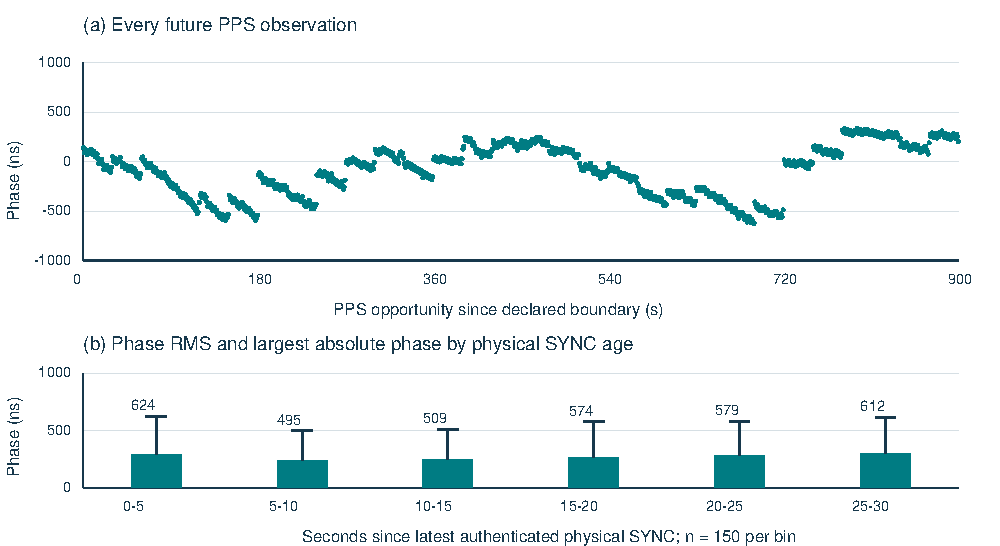
\includegraphics[width=0.88\linewidth]{phase-results.pdf}
\caption{Complete declared .288 validation. (a) All 900 delivered-model phases
at GNSS PPS inputs; the vertical scale includes $\pm1$ \us{}. (b) RMS bars and
maximum-absolute caps in six physical-SYNC-age bins, each with 150 observations.
No tail or interval is removed.}
\label{fig:phase}
\end{figure}
The phase scatter is visibly correlated across updates, consistent with a
shared causal prediction rather than 900 independent replications. The full
269.140 ns RMS, rather than the 251.809 ns centered SD, is the principal phase
summary after the independently frozen prior.
\clearpage

\section{What the interval results establish}
\subsection{Physical SYNC age and usable-map age}
Two clocks of age matter. Physical-SYNC age measures time since the most recent
authenticated physical SYNC, even while its FOLLOW is still in flight.
Accepted-pair age measures time since the SYNC belonging to the map's last
committed pair. Resetting the first age does not magically update the delivered
clock. During FOLLOW latency, the receiver still extrapolates the previous
map. Keeping these coordinates separate avoids making early-in-interval
performance look artificially fresh.

\begin{center}\small
\begin{tabular}{@{}lrrrrrr@{}}\toprule
Physical SYNC age (s)&0--5&5--10&10--15&15--20&20--25&25--30\\\midrule
PPS observations&150&150&150&150&150&150\\
Phase RMS (ns)&290.580&232.961&246.404&263.105&280.258&295.679\\
Maximum absolute (ns)&624&495&509&574&579&612\\\bottomrule
\end{tabular}
\end{center}
All six RMS values remain below 296 ns. There is no missing physical-age bin;
none of the primary observations had unknown age or physical-SYNC age at least
30 s. Separately, 91 samples had accepted-pair age at least 30 s, because a new
SYNC preceded its completed FOLLOW. Those samples had 311.897 ns RMS and
617 ns maximum. Their inclusion demonstrates that the low aggregate RMS does
not simply discard the previous-map portion of a precision interval.

This is stronger evidence for the tested sparse clock than a low fit residual
at packet arrival. It is still sampled, calibrated evidence from one future
window. No outage or extended holdover performance follows from six well-filled
bins under continuing successful updates. Source permission and the original
physical/context expiration fences remain necessary even when extrapolation
looks smooth.

\subsection{Bandwidth choice and the scope of ``best observed''}
Within B283's matched SF7/CR4/6 screen, 500 kHz had the lower observed centered
endpoint scatter. In B285, the pooled descriptive SDs across two recovery
streams were 2227.904, 2663.568, 1619.841, 819.229 and 218.137 ns from low to
high bandwidth. The increase from 41.67 to 62.5 kHz and the tiny per-stream
populations prevent a monotonic law. In particular, each stream's 500 kHz
arm had only one accepted pair, and the pooled two-pair SD is not a stable
noise estimate. Pooling cannot restore a missing complete forward/reverse block.

The final .288 run is the strongest complete, independently PPS-witnessed
delivered-model population selected here: 269.140 ns RMS over all 900 declared
future opportunities. Calling it the best complete observed result is a
statement about this evidence population. Its RMS cannot be ranked as the
same statistic as raw pair centered SD, in-sample link-fit RMS, future-pair
consistency or time deviation in other work. The incomplete .287 subset even
has a smaller conditional RMS; its missing opportunities prevent substituting
it as the primary result.

\subsection{Availability beyond the final T096 window}
The .288 window does not erase context turnover or heterogeneous service gaps.
A separate 1800-snapshot extension on a different receiver retained all snapshots
but reported LoRa availability in only 267; its 265--1512 ns internal fit
consistency had no independent phase witness. Such observations motivate
availability and handover qualification, not a transfer of the T096 result
to another target. Similarly, later source/receiver images share wire fields
without inheriting the measured .288 accuracy.
\clearpage

\section{Limits, reproducibility and next measurements}
The central identifiability limit is one-way transfer: a clock offset, a fixed
endpoint delay and propagation appear together. A constant prior can make
local model phase agree with a prior bench reference while leaving portable
UTC accuracy unresolved. A complete error budget would need independent
source uncertainty, GNSS input/capture delay, TX-marker-to-RF delay,
RX-detection delay, antenna/cable paths and the actual output path. The
present data do not identify each term. A low timer tick, MAC validity or a
checksum is insufficient evidence of timing accuracy.

The result also leaves environmental and service questions open. There is one
complete final window, one earlier four-pair calibration, no controlled
bandwidth-by-distance campaign, no field coverage distribution, no measured
EIRP and no interference/thermal population. Repeated held-out windows across
placements and temperatures would test calibration stability. A common clock
and external time-interval instrument at transmitter/receiver outputs would
separate input-model agreement from independently measured output error.
A prespecified channel/PHY matrix with sufficient repetitions would be needed
to compare fixed and hopped operation while retaining failed rendezvous and
all packet offers. These are proposed measurements, not work performed here.

The implementation boundary also matters. The fixed-profile cap is RAM-only
per boot; unknown source age remains unknown; LoRa observations do not create
BLE grandmaster, relay or USB timing authority. A longer observation lease is
not a promise of delivery or a calibrated uncertainty. Continuous receive can
simplify timing association, but its energy consumption has not been measured
in this experiment. These qualifications leave the finite result useful:
a sparse, authenticated one-way clock can retain sub-microsecond sampled
phase through its 30-second cycle in this calibrated T096 configuration.

\subsection{Reproducible selected evidence}
The accompanying \code{papers/lora-sparse-timing/} directory contains canonical
LaTeX/PDF, 900 .288 and 215 .287 opportunity rows, all 31 selected bandwidth
pairs with per-context offer counts, and the four calibration phases.
The standard-library analyzer recomputes means, uncentered RMS, centered SD,
nearest-rank absolute P99, maxima, both age populations, prior median and
packet airtime accounting. The vector plot draws every .288 observation.
Provenance records the selected private-input hashes and redactions; no raw
console log, key, enrollment, image or physical identity is redistributed.
The public derivatives reproduce the reported statistics, not private raw
capture extraction or physical calibration. Source snapshots distinguish the
measured .288 image from the later compatible wire reference; edition hashes
establish document identity, not accuracy.

\textbf{Author-review status and licensing.} This is a draft for Jonathan
Yantis to review before any public publication. The manuscript, original
figures and original selected datasets are CC BY 4.0, credited to Jonathan
Yantis; original analysis code is MIT. AI assistance supported evidence
organization, analysis-code preparation and drafting; the author retains
responsibility for interpretation and approval. No new hardware operations or
experiments were performed to prepare this retrospective.

\begin{thebibliography}{9}\small
\bibitem{longshot} C. G. Ramirez, A. Sergeyev, A. Dyussenova, and B. Iannucci,
``LongShoT: Long-Range Synchronization of Time,'' \emph{IPSN}, pp. 289--300,
2019. \href{https://doi.org/10.1145/3302506.3310408}{doi:10.1145/3302506.3310408}.
\bibitem{rinaldi} S. Rinaldi, E. Mondini, P. Ferrari, A. Flammini, and E. Sisinni,
``LoRa/LoRaWAN Time Synchronization: A Comprehensive Analysis, Performance
Evaluation, and Compensation of Frame Timestamping,'' \emph{Future Internet},
18(2), 80, 2026. \href{https://doi.org/10.3390/fi18020080}{doi:10.3390/fi18020080}.
\bibitem{mueller} P. M\"uller, D. Berger, and L. Sarperi, ``Nanosecond Time
Synchronization over a 2.4 GHz Long-Range Wireless Link,'' \emph{Sensors},
25(7), 1961, 2025. \href{https://doi.org/10.3390/s25071961}{doi:10.3390/s25071961}.
\end{thebibliography}
\end{document}
